\documentclass[12pt]{article}
\usepackage{amsmath}
\usepackage{graphicx}
\usepackage{amsfonts}
\usepackage{float}
\usepackage{geometry}
\usepackage{hyperref}
\usepackage{subcaption}
\geometry{a4paper, margin=1in}

\title{Actor-Critic Reinforcement Learning in MuJoCo}
\author{
    Mark Doughten [MD1875] \\
    Vijayendra Sai Chennareddy [VC545] \\
    Shubham Patil [SP2484]
}
\date{\today}
\begin{document}
\maketitle

\section{Introduction}
This report outlines the implementation of an Actor-Critic reinforcement learning (RL) framework a MuJoCo simulation environment. The objective is training a robot on the environment and understanding how it can reach the goal. This paper describes how this is achieved using neural networks for policy learning and value estimation with a reward function designed to encourage goal seeking. The transition function outlines the expected behavior. The transition function is defined as follows:

\begin{align*}
\dot{x}_{t+1} &= \dot{x}_t + (f_{x,t} - \rho_{x,t}) \Delta t, \\
\dot{y}_{t+1} &= \dot{y}_t + (f_{y,t} - \rho_{y,t}) \Delta t, \\
x_{t+1} &= x_t + \dot{x}_t \Delta t, \\
y_{t+1} &= y_t + \dot{y}_t \Delta t.
\end{align*}

where \( \rho_{x,t} \) and \( \rho_{y,t} \) are small independent noises, sampled from \( \mathcal{N}(0, 0.1) \) at each time step \( t \), and \( \Delta t \) is set to 0.1 seconds. We assume here that the robot has a mass of 1~kg. You can interpret the force noises as air resistance or random friction (although air resistance should scale up as a function of velocity).

\section{Environment}
The environment is a 3D course simulated in MuJoCo, featuring obstacles and boundaries. The robot is subjected to forces in the \(x\)- and \(y\)-directions. The actor applies a force on the robot based on the current policy. The reward function incentives reaching the goal and penalizes wasting time. The initial state is obtained by sampling the
position of the robot uniformly in the workspace of the robot, and setting
its initial velocity to 0. An example of how the points were selected during a batch training session, showing the initial starting positions are random. 

\begin{figure}[H]
    \centering
    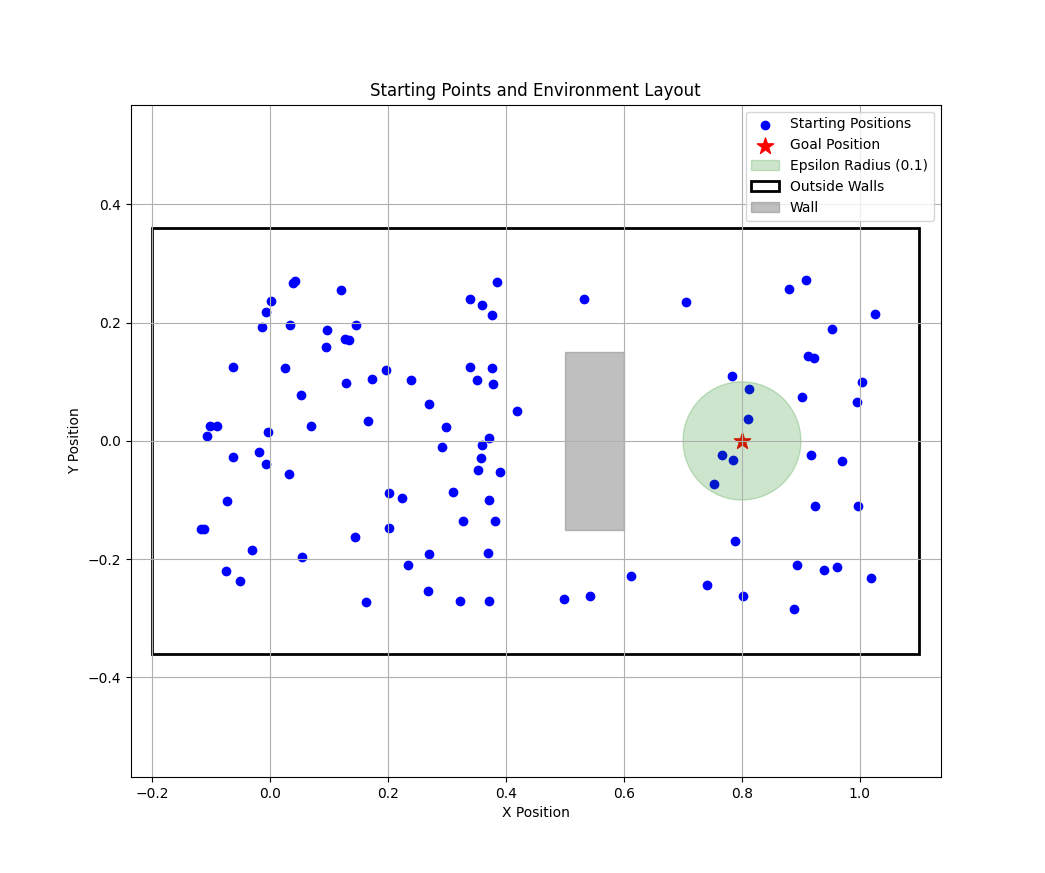
\includegraphics[width=0.8\textwidth]{report/images/environment.png}
    \caption{Spawn locations during the training process.}
    \label{fig:trajectory}
\end{figure}

The goal position is fixed on (0.8, 0.0) and the epsilon is 0.1. Overall, this was a challenging configuration since the robot needs to learn how to travel above or below the obstacle in the middle. It makes a simple reward function like distance to the goal not beneficial since the robot will find an optimal point on the side closest. 

\section{Actor-Critic Model}

The framework for the Actor-Critic model is based on Hado van Hasselt's lecture. 

\begin{figure}[H]
    \centering
    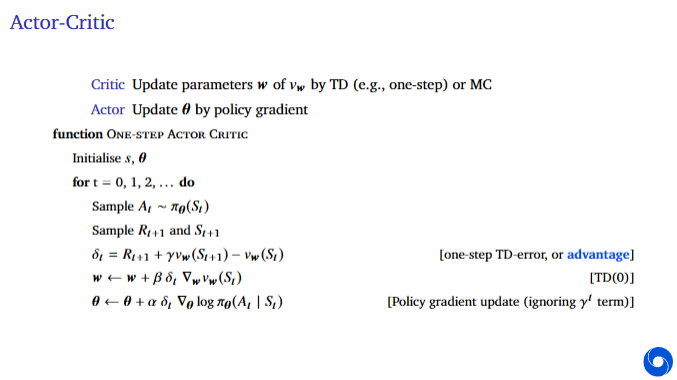
\includegraphics[width=0.8\textwidth]{report/images/slide40.PNG}
    \caption{Pseudocode}
    \label{fig:slide40}
\end{figure}

The Actor-Critic architecture comprises two neural networks:
\begin{itemize}
    \item \textbf{Actor Network:} Outputs an action in the form of a mean (\(\mu\)) and standard deviation (\(\sigma\)) for each step in the episode.
    \item \textbf{Critic Network:} Estimates the value function and provides feedback to improve the actor's policy.
\end{itemize}

\subsection{Actor Network}
The actor network processes the robot's state (\(x, y, v_x, v_y\)) through three fully connected layers. The output represents the mean and standard deviation for a Gaussian policy, \(a\) is the action vector consisting of control forces in the \(x\)- and \(y\)-directions.

\begin{equation}
\pi(a|s) \sim \mathcal{N}(\mu(s), \sigma(s)),
\end{equation}

\begin{figure}[H]
    \centering
    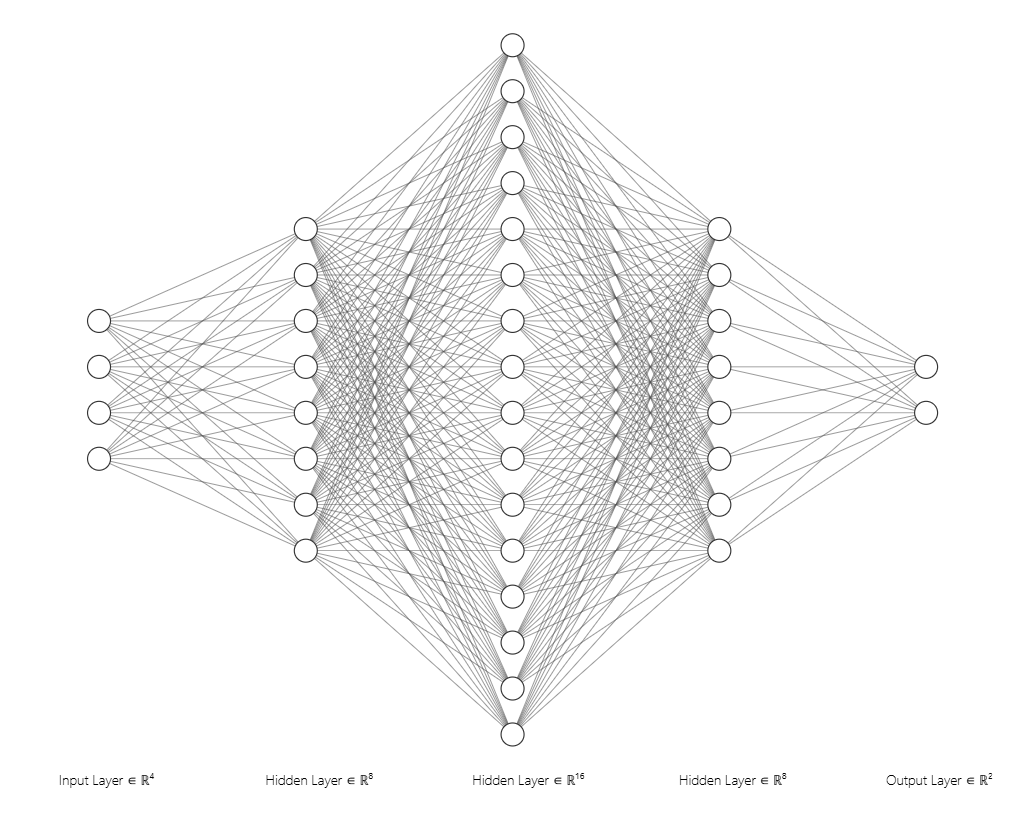
\includegraphics[width=0.8\textwidth]{report/images/nn.png}
    \caption{Actor Network Architecture}
    \label{fig:actor_network}
\end{figure}

\subsection{Critic Network}
The critic network uses the same input as the actor and a single scalar value that represents the estimated state value \(V(s)\). This value guides the actor policy by estimating the advantage of actions. The two networks work together to achieve the optimal actions based on the policy gradient.

\subsection{Loss Functions}
\begin{itemize}
    \item \textbf{Actor Loss:} Encourages actions that maximize expected rewards:
    \[
    L_\text{actor} = -\mathbb{E}[\log\pi(a|s) \cdot \text{Advantage}(s, a)].
    \]
    \item \textbf{Critic Loss:} Minimizes the temporal difference (TD) error:
    \[
    L_\text{critic} = \frac{1}{2} (\text{TD Target} - V(s))^2.
    \]
\end{itemize}

\begin{figure}[H]
    \centering
    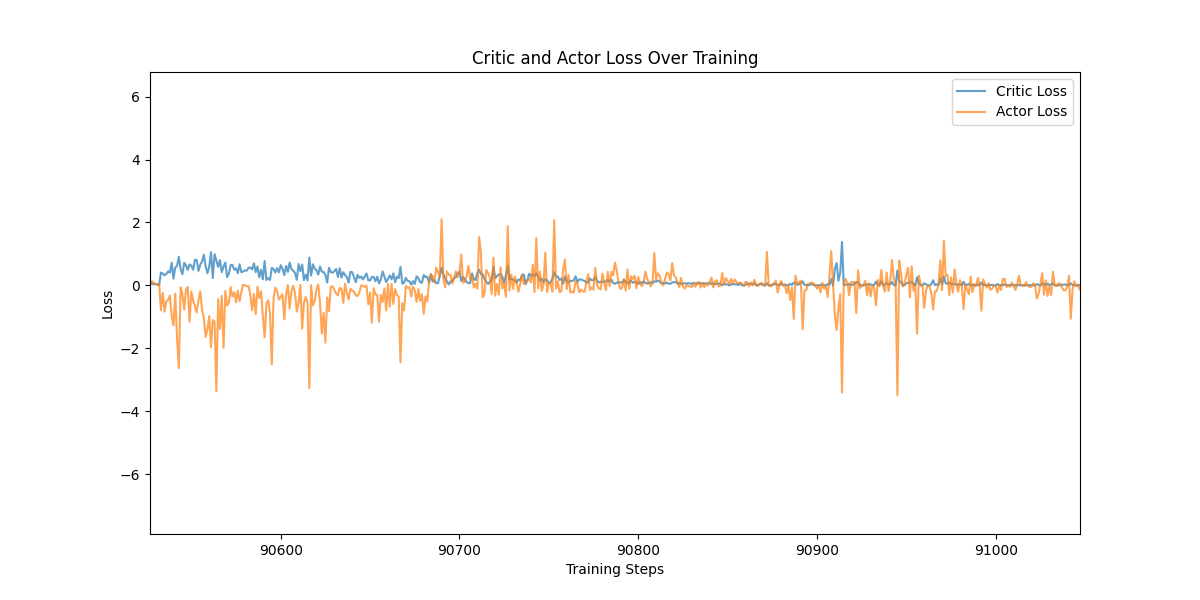
\includegraphics[width=0.8\textwidth]{report/images/loss.png}
    \caption{Recorded loss during a training session.}
    \label{fig:trajectory}
\end{figure}

\section{Training}

\subsection{Reward Function}
The reward function balances three objectives:
\begin{itemize}
    \item \textbf{Distance to Goal:} Encourages progress toward the goal with a linear penalty proportional to the distance.
    \item \textbf{Time Penalty:} Incentives finding the goal quicker during each episode. 
\end{itemize}

\subsection{Method}
The training process allows the user to set the duration and the number of steps. In our case, we typically set the number of steps to 1800 and episodes vary based on the session. While we can train in batch, a user can view a training session in between the batches to see the progression. Likewise, we have the option to run from a fixed point and 
The training loop iteratively performs the following steps:
\begin{enumerate}
    \item Initialize the state \(s_0\).
    \item Use the actor network to sample an action \(a_t\).
    \item Apply \(a_t\) in the environment and record the next state \(s_{t+1}\) and reward \(r_t\).
    \item Compute the temporal difference (TD):
    \[\text{TD} = r_t + \gamma V(s_{t+1}),\]
    where $\gamma=0.99$ is the discount factor.
    \item Backpropagation to the actor and critic networks using their respective loss functions.
\end{enumerate}

\section{Results}

\subsection{Learning Curve}
The model achieves consistent improvements in reward over episodes. Figure \ref{fig:learning_curve} illustrates the average reward per episode during training.

\begin{figure}[H]
    \centering
    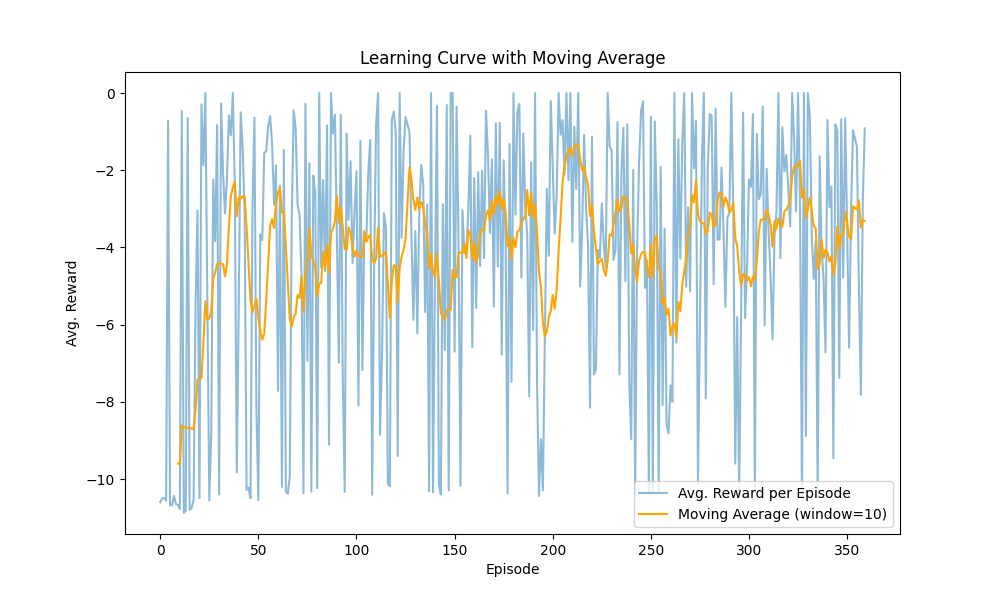
\includegraphics[width=0.8\textwidth]{report/images/learning.png}
    \caption{Average reward per episode during training.}
    \label{fig:learning_curve}
\end{figure}

\section{Conclusion}
The Actor-Critic reinforcement learning framework demonstrates effective navigation to the goal in a 3D simulated environment. Future work could involve extending this approach for submersibles and obstacle avoidance using sensors.

\begin{thebibliography}{}
\raggedright

\bibitem{vanHasselt} 
van Hasselt, H. Lecture 9: Policy Gradients and Actor Critics; UCL, 2021. 

\bibitem{jaramillo} 
Jaramillo-Martínez, R.; Chavero-Navarrete, E.; Ibarra-Pérez, T. Reinforcement-Learning-Based Path Planning: A Reward Function Strategy. \textit{Applied Sciences} \text{2024}, \text{14} (17), 7654. \url{https://doi.org/10.3390/app14177654}.

\bibitem{larsen} 
Larsen, T. N.; Teigen, H. Ø.; Laache, T.; Varagnolo, D.; Rasheed, A. Comparing Deep Reinforcement Learning Algorithms’ Ability to Safely Navigate Challenging Waters. \textit{Frontiers in Robotics and AI} \text{2021}, \text{8}, 738113. \url{https://doi.org/10.3389/frobt.2021.738113}.

\bibitem{manuelli} 
Manuelli, L.; Florence, P. Reinforcement Learning for Autonomous Driving Obstacle Avoidance using LIDAR. \textit{Massachusetts Institute of Technology.} Available online: \url{https://www.peteflorence.com/ReinforcementLearningAutonomousDriving.pdf}.

\end{thebibliography}
\end{document}